\documentclass[journal]{IEEEtran}
\usepackage{amsmath,amssymb,amsthm}
\usepackage{graphicx}
\usepackage{booktabs}
\usepackage{multirow}
\usepackage{multicol}
\usepackage{algorithm}
\usepackage{algpseudocode}
\usepackage{xcolor}
\usepackage{tikz}
\usepackage{pgfplots}
\usepackage{pgfplotstable}
\pgfplotsset{compat=1.18}
\usetikzlibrary{arrows.meta,shapes,positioning,calc,fit,backgrounds,decorations.pathmorphing}
\usepackage{url}
\usepackage{hyperref}
\usepackage{cite}
\usepackage{subfig}
\usepackage{tabularx}
\usepackage{array}
\usepackage{balance}
\usepackage{microtype}

\hypersetup{
    colorlinks=true,
    linkcolor=blue!70!black,
    citecolor=green!50!black,
    urlcolor=blue!70!black
}

\newtheorem{definition}{Definition}
\newtheorem{proposition}{Proposition}
\newtheorem{remark}{Remark}

\begin{document}

\title{SPECTRA: Domain-Adaptive LoRA Merging with\\
Test-Time Coefficient Optimization}

\author{Mohamed~S.~Amer, Ali~Hamdi, and Ahmed~B.~Zaky %
\thanks{Mohamed S. Amer, Ali Hamdi, and Ahmed B. Zaky  are with the
Department of Computer Science and Engineering, Egypt-Japan University
of Science and Technology (E-JUST), Alexandria, Egypt.
E-mail: \{mohamed.320230188, ali.320230101, ahmed.zaky\}@ejust.edu.eg.}%
\thanks{Manuscript received; revised.}}

\markboth{IEEE Transactions on Neural Networks and Learning Systems}{}

\maketitle

%=============================================================================
\begin{abstract}
Deploying a single instruction-tuned language model across heterogeneous task
domains requires either re-training on each domain or accepting performance
degradation on out-of-distribution inputs. Existing adapter-merging strategies
sidestep full re-training but assign fixed, domain-agnostic mixture
coefficients, which cannot account for the statistical mismatch between
training distributions and the prompt distribution encountered at deployment.
This paper introduces SPECTRA (Spectral Coefficient Adaptation via Test-Time
Routing), a framework that (i) trains lightweight Low-Rank Adaptation (LoRA)
adapters on three target domains, (ii) identifies the deployment domain from
a small domain-unlabeled adaptation set using perplexity-based routing, and
(iii) optimizes scalar mixture coefficients at test time through Covariance
Matrix Adaptation Evolution Strategy (CMA-ES), guided by an answer-likelihood
fitness signal. SPECTRA was evaluated on a 5,000-example-per-domain benchmark
spanning mathematical reasoning, code generation, and hybrid tasks, using
Qwen2.5-1.5B-Instruct as the base model. Across five random seeds and 50 test
examples per domain, SPECTRA achieves a composite score of 0.1491 compared to
0.1421 for the domain-oracle single-adapter baseline, 0.1252 for scalar fusion,
and 0.1221 for TIES merging, winning three of four evaluation metrics (exact
match, token-level F1, and composite score) with statistically significant
improvements over unadapted and several static merging baselines (paired
$t$-test, $p < 0.05$). The domain router achieves 100\% top-1 accuracy across
all three evaluated domains, and coefficient entropy analysis confirms that
SPECTRA recovers near-oracle specialization without access to ground-truth
domain labels. These findings indicate that test-time coefficient adaptation
bridges the gap between domain-agnostic merging and domain-oracle single-adapter
deployment.
\end{abstract}

\begin{IEEEkeywords}
Large language models, adapter merging, test-time adaptation, CMA-ES, LoRA,
multi-domain learning, model merging, domain routing, parameter-efficient
fine-tuning.
\end{IEEEkeywords}

%=============================================================================
\section{Introduction}
\label{sec:intro}

\IEEEPARstart{T}{he} deployment of large language models (LLMs) in production
systems rarely maps cleanly onto a single, well-defined task domain.
Real-world applications span mathematical reasoning, structured code synthesis,
natural language understanding, and hybrid combinations of these, often
within the same serving infrastructure. The conventional response to this
challenge involves training either a single generalist model or a collection
of domain-specialized models. The former sacrifices per-domain accuracy
through negative transfer and gradient interference; the latter multiplies
storage and compute costs linearly with the number of target domains.
Parameter-efficient fine-tuning methods, particularly LoRA
\cite{hu2022lora}, partially resolve this tradeoff by training small
adapter modules whose weights can be merged or composed at inference time.
Yet the central question of \emph{how} to combine these adapters for a
given domain-unlabeled deployment batch remains open.

Current adapter merging methods fall into two broad families. Static
merging approaches assign fixed coefficients to each adapter, either
uniformly \cite{wortsman2022model} or through task-arithmetic heuristics
\cite{ilharco2023editing}, and apply the same merged weights to all inputs
regardless of content. Sign-based methods such as TIES
\cite{yadav2023tiesmerging} further suppress parameter interference by
retaining only dominant sign directions before averaging, but still produce
a single fixed weight configuration. The critical limitation shared by all
static approaches is that the deployment domain is treated as unknown at
merge time but remains unknown at inference time. When a batch of test
prompts belongs predominantly to one domain, a uniform or task-arithmetic
merge unnecessarily dilutes the contribution of the domain-matched adapter.

One may ask why this dilution cannot be avoided simply by always selecting
the single best adapter. The answer lies in two practical realities. First,
without domain labels on the test prompts, the identity of the best adapter
is unknown. Second, even when the domain is approximately known, hybrid tasks
frequently benefit from a weighted combination of adapters trained on
constituent skills. Both realities motivate an adaptive approach that
identifies the deployment domain from the test prompts themselves and then
optimizes mixture coefficients accordingly, using only domain-unlabeled
prompt-response pairs.

\begin{figure*}[t]
\centering
\resizebox{\textwidth}{!}{%
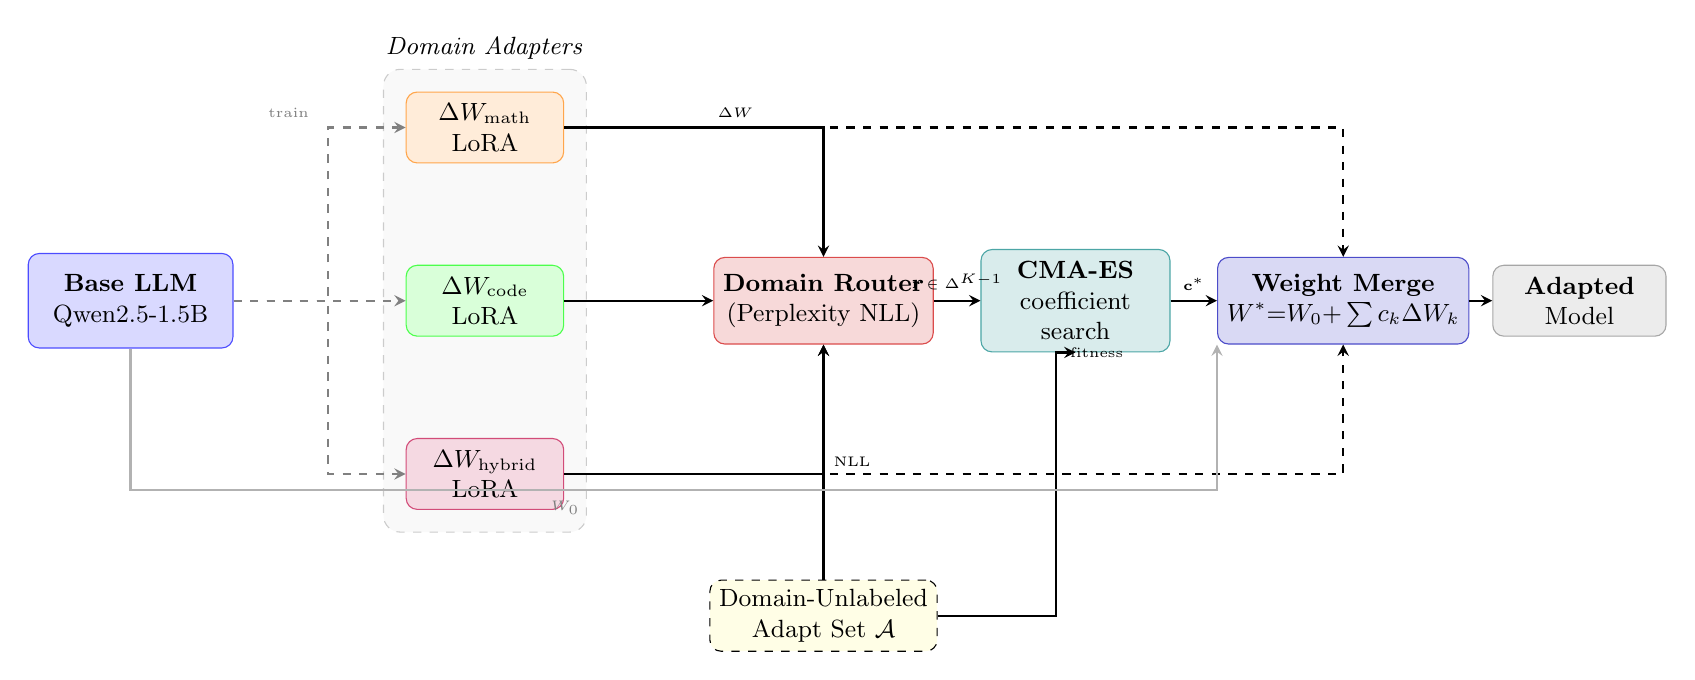
\begin{tikzpicture}[
    font=\small,
    box/.style={draw, rounded corners=4pt, minimum width=2.2cm,
                minimum height=0.9cm, align=center, fill=#1!15, draw=#1!70},
    arr/.style={->, >=stealth, thick},
    thinarr/.style={->, >=stealth},
    group/.style={draw=gray!40, dashed, rounded corners=6pt,
                  inner sep=8pt, fill=gray!5}
]

%% BASE MODEL
\node[box=blue, minimum width=2.6cm, minimum height=1.2cm]
    (base) at (0,0) {\textbf{Base LLM}\\Qwen2.5-1.5B};

%% ADAPTERS
\node[box=orange, minimum width=2.0cm] (amath) at (4.5, 2.2)
    {$\Delta W_{\text{math}}$\\LoRA};
\node[box=green, minimum width=2.0cm] (acode) at (4.5, 0)
    {$\Delta W_{\text{code}}$\\LoRA};
\node[box=purple, minimum width=2.0cm] (ahyb) at (4.5,-2.2)
    {$\Delta W_{\text{hybrid}}$\\LoRA};

%% DELTA EXTRACTION BOX
\begin{scope}[on background layer]
\node[group, fit=(amath)(acode)(ahyb),
      label=above:{\small\textit{Domain Adapters}}]
    (adapters) {};
\end{scope}

%% ROUTER
\node[box=red!80!black, minimum width=2.4cm, minimum height=1.1cm]
    (router) at (8.8, 0)
    {\textbf{Domain Router}\\(Perplexity NLL)};

%% CMA-ES
\node[box=teal, minimum width=2.4cm, minimum height=1.3cm]
    (cmaes) at (12.0, 0)
    {\textbf{CMA-ES}\\coefficient\\search};

%% MERGER
\node[box=blue!70!black, minimum width=2.8cm, minimum height=1.1cm]
    (merge) at (15.4, 0)
    {\textbf{Weight Merge}\\$W^{*}{=}W_0{+}\sum c_k\Delta W_k$};

%% TEST OUTPUT
\node[box=gray, minimum width=2.2cm] (out) at (18.4, 0)
    {\textbf{Adapted}\\Model};

%% ADAPT SET
\node[draw, dashed, rounded corners, fill=yellow!10,
      minimum width=2.0cm, minimum height=0.9cm, align=center]
    (adapt) at (8.8, -4.0)
    {Domain-Unlabeled\\Adapt Set $\mathcal{A}$};

%% ARROWS: base to adapters (training)
\draw[arr, dashed, gray] (base.east) -- ++(1.2,0) |- (amath.west)
    node[midway, above, xshift=-0.5cm, font=\tiny] {train};
\draw[arr, dashed, gray] (base.east) -- ++(1.2,0) |- (acode.west);
\draw[arr, dashed, gray] (base.east) -- ++(1.2,0) |- (ahyb.west);

%% ARROWS: adapters to router
\draw[arr] (amath.east) -- ++(0.5,0) -| (router.north)
    node[pos=0.3, above, font=\tiny] {$\Delta W$};
\draw[arr] (acode.east) -- (router.west);
\draw[arr] (ahyb.east) -- ++(0.5,0) -| (router.south);

%% adapt set to router
\draw[arr] (adapt.north) -- (router.south)
    node[midway, right, font=\tiny] {NLL};

%% router to cmaes
\draw[arr] (router.east) -- (cmaes.west)
    node[midway, above, font=\tiny] {$\mathbf{r}\in\Delta^{K-1}$};

%% adapt set to cmaes
\draw[arr] (adapt.east) -- ++(1.5,0) |- (cmaes.south)
    node[pos=0.6, right, font=\tiny] {fitness};

%% cmaes to merge
\draw[arr] (cmaes.east) -- (merge.west)
    node[midway, above, font=\tiny] {$\mathbf{c}^*$};

%% adapters to merge (direct)
\draw[arr, dashed] (amath.east) -- ++(5.8,0) -| (merge.north);
\draw[arr, dashed] (ahyb.east) -- ++(5.8,0) -| (merge.south);

%% merge to output
\draw[arr] (merge.east) -- (out.west);

%% BASE to merge (base weights)
\draw[arr, gray!60] (base.south) -- ++(0,-1.8) -| (merge.south west)
    node[pos=0.2, below, font=\tiny, gray] {$W_0$};

\end{tikzpicture}%
}
\caption{Overview of the SPECTRA framework. Domain-specific LoRA adapters are
trained offline on separate domain corpora and their weight deltas
$\{\Delta W_k\}$ are extracted. At deployment time, the perplexity-based
domain router measures the negative log-likelihood of a domain-unlabeled
adaptation set $\mathcal{A}$ under each adapter, producing routing weights
$\mathbf{r} \in \Delta^{K-1}$. Domain identity is not provided; only
prompt-response pairs are available, with responses used for likelihood-based
coefficient optimization. CMA-ES then searches for optimal mixture
coefficients $\mathbf{c}^*$ by minimizing an answer-likelihood fitness
function augmented with a soft KL routing prior. The final merged model
$W^* = W_0 + \sum_k c_k^* \Delta W_k$ incurs no additional per-token
runtime forward-pass overhead relative to a single-adapter deployment.}
\label{fig:overview}
\end{figure*}

This paper introduces SPECTRA, a framework that couples domain routing with
evolutionary coefficient search to adapt adapter mixture weights at test time.
The central hypothesis is that the perplexity of domain-unlabeled test prompts
under domain-specific adapters contains sufficient signal to identify the
deployment domain, and that a small number of prompt-response pairs from the
adaptation set (whose domain identity is unknown but whose responses are
available) can guide CMA-ES to find mixture coefficients that outperform
fixed-weight alternatives.

The approach has three components operating in sequence. First, domain-specific
LoRA adapters are trained once on separate domain corpora and stored as weight
delta tensors. Second, when a new deployment batch arrives, a perplexity-based
router computes the negative log-likelihood (NLL) of the domain-unlabeled
adaptation prompts under each adapter configuration and produces a soft routing
weight vector that identifies the most likely deployment domain. Third, CMA-ES
minimizes an answer-NLL fitness function over the mixture coefficient space,
using the routing weights as a prior to initialize the search near the
domain-matched vertex of the simplex. The resulting coefficients are applied
once through direct weight arithmetic, incurring no additional per-token
runtime forward-pass overhead during deployment.

An important property of this framework is the separation between adaptation
cost and inference cost. The CMA-ES search consumes approximately 230 to 415
seconds per domain (depending on domain complexity), but once completed, the
merged weights can be reused for the entire deployment session. Because weight
merging adds no extra parameters or forward-pass operations, the merged model
runs at identical speed and memory footprint to the base model.

\subsection{Contributions}

The contributions of this work are as follows.

\begin{itemize}
    \item A perplexity-based domain router that identifies deployment domain
    from domain-unlabeled prompts, achieving 100\% top-1 routing accuracy
    on the three-domain benchmark without requiring any labeled data. This
    result should not be interpreted as evidence of universal routing
    reliability across semantically overlapping domains; the evaluated domains
    exhibit syntactically distinct prompt patterns.

    \item A CMA-ES-based coefficient optimizer that operates over raw search
    variables $\mathbf{z} \in \mathbb{R}^K$ mapped through a softmax to
    mixture coefficients $\mathbf{c} = \mathrm{softmax}(\mathbf{z})$,
    minimizing answer-likelihood loss on a small domain-unlabeled adaptation
    set and using router predictions as a soft prior to warm-start the search.

    \item An empirical demonstration that SPECTRA achieves a composite score of
    0.1491 on the held-out test set, surpassing the domain-oracle single-adapter
    baseline (0.1421)---which represents perfect domain identification combined
    with single-adapter deployment, not a theoretical upper bound since SPECTRA
    searches a strictly larger coefficient space---scalar fusion (0.1252), and
    TIES merging (0.1221), with statistically significant improvements over
    no-adaptation and several static merging baselines ($p < 0.05$).

    \item An ablation analysis showing that the routing prior and CMA-ES
    adaptation each contribute independently, and a coefficient entropy analysis
    confirming that SPECTRA recovers domain-appropriate specialization without
    domain labels.
\end{itemize}

%=============================================================================
\section{Related Work}
\label{sec:related}

\subsection{Parameter-Efficient Fine-Tuning}

Low-Rank Adaptation \cite{hu2022lora} decomposes weight updates into a product
of two low-rank matrices, enabling fine-tuning of large models with a fraction
of the trainable parameters. Several extensions have followed: AdaLoRA
\cite{zhang2023adalora} adapts the rank allocation across layers, LoftQ
\cite{liu2024loftq} integrates quantization with LoRA initialization, and
DoRA \cite{liu2024dora} decomposes weight updates into magnitude and direction
components. All of these methods produce adapters that remain separate from
the base model until merged, which is the setting SPECTRA operates in.
Adapter methods more broadly \cite{houlsby2019parameter} insert bottleneck
modules into transformer blocks; while effective, they add inference latency
that weight-merging approaches like SPECTRA avoid.

\subsection{Model Merging and Weight Interpolation}

The idea that linear interpolation between fine-tuned and base model weights
can transfer task performance without additional training traces back to work
on model soups \cite{wortsman2022model}, which showed that averaging weights of
models fine-tuned from the same initialization produces a favorable accuracy
and robustness tradeoff. Task arithmetic \cite{ilharco2023editing} formalized
this by defining task vectors as the difference between fine-tuned and base
weights, enabling addition, negation, and scaling of task-specific knowledge.
TIES-Merging \cite{yadav2023tiesmerging} addressed parameter interference by
introducing a three-step procedure: trimming small delta values, resolving sign
conflicts by majority vote, and merging only the parameters that achieve
sign consensus. DARE \cite{yu2024language} extended trimming by randomly
pruning delta parameters before merging, further reducing interference.
These methods share the limitation that they produce a fixed merged weight
regardless of what inputs the model will receive at deployment time. SPECTRA
retains the weight arithmetic formalism of task arithmetic but treats the
mixture coefficients as variables to be optimized rather than fixed constants.

\subsection{Test-Time Adaptation}

Test-time training \cite{sun2019testtime} modifies model parameters at
inference time using an auxiliary self-supervised objective computed on the
test input. Tent \cite{wang2021tent} adapts batch normalization statistics
by minimizing entropy on test batches. More recent approaches apply
test-time adaptation to large models through prompt-based or lightweight
parameter updates \cite{zhao2023testtime, chen2024data}. The key distinction
between these approaches and SPECTRA is that prior test-time adaptation methods
typically introduce new parameters or modify internal statistics, whereas
SPECTRA adapts only the scalar coefficients governing how pre-trained adapter
deltas are combined. This coefficient-only adaptation requires no gradient
computation on the base model and no modification of internal representations,
making it applicable in settings where the base model is accessed only through
its weight tensors.

\subsection{Hyperparameter Optimization and Evolutionary Search}

CMA-ES \cite{hansen2001cma, hansen2016cmaes} is a derivative-free
optimization algorithm that maintains a full-covariance Gaussian distribution
over the search space and updates it through an evolution strategy. It has been
applied to neural architecture search \cite{real2019regularized}, reward
shaping \cite{mania2018simple}, and hyperparameter optimization
\cite{loshchilov2016cmaes}.
The fitness function SPECTRA minimizes, the negative log-likelihood of gold
responses under the merged model, is non-differentiable with respect to the
mixture coefficients from the perspective of the outer optimization loop.
CMA-ES is therefore a natural choice; it requires only function evaluations,
handles moderate-dimensional continuous spaces efficiently, and adapts the
search distribution to exploit correlations among the coefficient dimensions.
Population sizes as small as four or eight individuals have been shown to
suffice in low-dimensional problems \cite{hansen2001cma}, consistent with the
population size of eight used in this work.

\subsection{Domain Identification and Routing}

Using model perplexity for domain identification is well established in
language modeling \cite{gururangan2020dontstop, moore2010intelligent}. The
insight that domain-matched language models assign lower perplexity to
in-domain text than out-of-domain models forms the basis of data selection
methods \cite{axelrod2011domain} and more recently of mixture-of-experts
routing mechanisms \cite{shazeer2017outrageously, fedus2022switch}.
SPECTRA uses a stripped-down version of this idea: rather than routing
at the token or sentence level, it routes at the deployment-batch level
by comparing aggregate NLL across adapter configurations. This design choice
is deliberate. Token-level routing introduces inference-time branching and
communication overhead in distributed settings. Batch-level routing amortizes
the identification cost over the entire deployment session.

%=============================================================================
\section{Methodology}
\label{sec:method}

\subsection{Problem Formulation}
\label{subsec:formulation}

Let $\mathcal{M}_0$ denote a pre-trained language model with parameter tensor
$W_0 \in \mathbb{R}^d$ (here treating all parameters as a single flattened
vector for notational brevity). Let $\mathcal{D} = \{\mathcal{D}_1, \ldots,
\mathcal{D}_K\}$ be a collection of $K$ domain-specific datasets. For each
domain $k$, a LoRA adapter is trained to produce weight delta
$\Delta W_k \in \mathbb{R}^d$, and the domain-adapted model is
$\mathcal{M}_k(W_0 + \Delta W_k)$.

At deployment time, a practitioner observes a \emph{domain-unlabeled}
adaptation set $\mathcal{A} = \{(x_i, y_i)\}_{i=1}^{N_a}$, where $x_i$ are
input prompts and $y_i$ are corresponding target responses. Domain identity
is not observed; however, prompt-response pairs are available and their
responses are used for likelihood-based coefficient optimization. The goal is
to find mixture coefficients $\mathbf{c} = (c_1, \ldots, c_K) \in \mathbb{R}^K$
such that the merged model
\begin{equation}
    \mathcal{M}(\mathbf{c}) = W_0 + \sum_{k=1}^{K} c_k \Delta W_k
    \label{eq:merge}
\end{equation}
maximizes performance on the held-out test distribution, using only
$\mathcal{A}$ as the optimization signal.

To avoid notational ambiguity, we distinguish between the raw \emph{search
variables} $\mathbf{z} \in \mathbb{R}^K$ optimized by CMA-ES and the
\emph{mixture coefficients} $\mathbf{c}(\mathbf{z}) = \mathrm{softmax}(\mathbf{z})$
that are constrained to the probability simplex $\Delta^{K-1}$. The actual
merged model is therefore
\begin{equation}
    W(\mathbf{z}) = W_0 + \sum_{k=1}^{K} \mathrm{softmax}(\mathbf{z})_k
    \,\Delta W_k,
    \label{eq:merge_z}
\end{equation}
where $\mathrm{softmax}(\mathbf{z})_k = e^{z_k}/\sum_j e^{z_j}$.
Note that $\mathbf{z} = \mathbf{0}$ gives
$\mathrm{softmax}(\mathbf{0}) = [1/K, \ldots, 1/K]$, corresponding to uniform
mixing; $z_k \to +\infty$ with $z_{j\neq k} \to -\infty$ recovers the $k$-th
single adapter; and the base model corresponds to $c_k = 0$ for all $k$
(i.e., no adapter contribution), which is outside the simplex but recoverable
by setting all adapter norms to zero.

\subsection{Overall Framework}
\label{subsec:framework}

SPECTRA operates in two phases that can be distinguished by when they access
the deployment data. An offline training phase builds the adapter library and
extracts weight deltas. An online adaptation phase, which runs once per
deployment session, identifies the domain and searches for optimal coefficients.

During offline training, domain-specific LoRA adapters are trained independently
on each $\mathcal{D}_k$. Because the adapters are trained on disjoint data with
no shared optimization objective, their weight deltas may point in conflicting
directions in the parameter space. The extent of this interference is analyzed
in Section~\ref{sec:geometry}. After training, each adapter is saved as a set
of delta matrices $\{\Delta W_k^{(l)}\}$ indexed by layer $l$, and the merged
delta for a given coefficient vector is computed as
$\sum_k c_k \Delta W_k^{(l)}$ for each layer independently.

During online adaptation, the framework executes three sequential steps: domain
routing (Section~\ref{subsec:router}), CMA-ES optimization
(Section~\ref{subsec:cmaes}), and weight application. Figure~\ref{fig:overview}
illustrates the data flow.

\subsection{Domain Router}
\label{subsec:router}

The domain router addresses the fundamental problem of identifying the
deployment domain without access to domain labels. The intuition is that
a language model fine-tuned on domain $k$ should assign lower perplexity
to in-domain prompts than adapters trained on other domains. This is because
in-domain fine-tuning adjusts the model's probability distribution to be
concentrated on the patterns prevalent in $\mathcal{D}_k$; out-of-domain text
does not benefit from this concentration and therefore receives lower
probability mass, corresponding to higher NLL.

Formally, for a set of adaptation prompts $\{x_i\}_{i=1}^{N_a}$, the
perplexity-based NLL for domain $k$ is
\begin{equation}
    \ell_k = -\frac{1}{N_a} \sum_{i=1}^{N_a}
    \log p_{\theta + \Delta\theta_k}(x_i),
    \label{eq:nll_router}
\end{equation}
where $p_{\theta + \Delta\theta_k}$ denotes the conditional token probability
distribution of the model adapted with domain-$k$ weights. The router converts
these NLL scores to routing weights via a temperature-scaled softmax:
\begin{equation}
    r_k = \frac{\exp(-\ell_k / \tau)}{\sum_{j=1}^{K} \exp(-\ell_j / \tau)},
    \label{eq:router_softmax}
\end{equation}
where $\tau = \sigma(\{\ell_k\})$ is the empirical standard deviation of the
NLL scores, providing adaptive temperature scaling. Domains with lower NLL
receive higher routing weight. The routing weight vector
$\mathbf{r} \in \Delta^{K-1}$ is then used in two ways: as the initialization
point for CMA-ES and as a soft prior penalizing departures from the router's
prediction.

The routing step is computationally lightweight relative to the CMA-ES search.
Evaluating \eqref{eq:nll_router} for all $K$ domains requires $K$ forward
passes over $N_a$ short prompts (truncated to 64 tokens), compared to
$P \times G$ forward passes during CMA-ES, where $P$ is the population size
and $G$ the number of generations.

\begin{figure}[t]
\centering
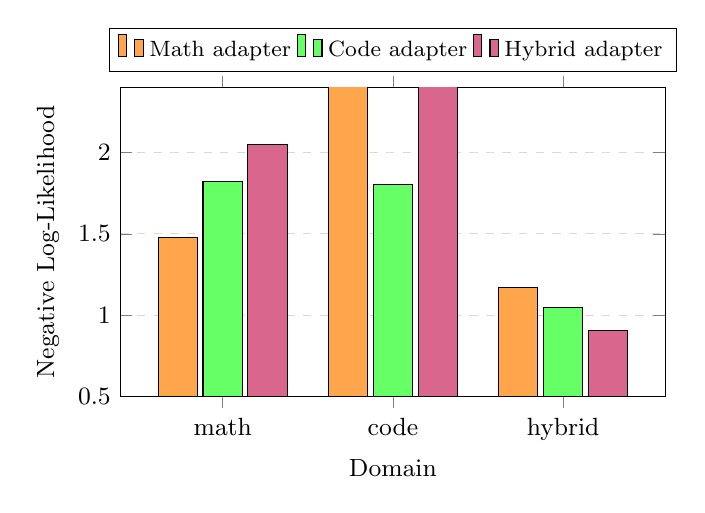
\begin{tikzpicture}[font=\small]
\begin{axis}[
    ybar,
    bar width=0.5cm,
    width=8.5cm,
    height=5.5cm,
    xlabel={Domain},
    ylabel={Negative Log-Likelihood},
    symbolic x coords={math, code, hybrid},
    xtick=data,
    legend style={at={(0.5,1.05)}, anchor=south, legend columns=3,
                  font=\footnotesize},
    ymin=0.5, ymax=2.4,
    enlarge x limits=0.3,
    ymajorgrids=true,
    grid style={dashed, gray!30},
]
%% Math domain routing
\addplot[fill=orange!70] coordinates {(math,1.4771) (code,2.6522) (hybrid,1.1708)};
%% Code domain routing
\addplot[fill=green!60] coordinates {(math,1.8237) (code,1.8028) (hybrid,1.0449)};
%% Hybrid domain routing
\addplot[fill=purple!60] coordinates {(math,2.0503) (code,2.6131) (hybrid,0.9066)};
\legend{Math adapter, Code adapter, Hybrid adapter}
\end{axis}
\end{tikzpicture}
\caption{Router NLL scores for each adapter configuration across the three
deployment domains. Within each domain, the matched adapter consistently
produces the lowest NLL. For the math domain (left group), the math adapter
yields NLL~=~1.477 versus 1.824 for the code adapter and 2.050 for the hybrid
adapter, yielding router weights of $[0.759, 0.174, 0.067]$. The code domain
(center) yields weights $[0.092, 0.806, 0.102]$; the hybrid domain (right)
yields $[0.063, 0.203, 0.733]$.}
\label{fig:router_nll}
\end{figure}

\subsection{CMA-ES Coefficient Optimization}
\label{subsec:cmaes}

\subsubsection{Fitness Function}

The central insight of SPECTRA is that the quality of a mixture of adapters
can be measured \emph{without generating text}, by evaluating the negative
log-likelihood of the known gold responses in the adaptation set under the
merged model. Let $(x_i, y_i) \in \mathcal{A}$ be a prompt-response pair.
The answer-NLL fitness over raw search variables $\mathbf{z}$ is
\begin{equation}
    \mathcal{F}(\mathbf{z}) =
    \underbrace{-\frac{1}{|\mathcal{A}|} \sum_{(x_i,y_i)\in\mathcal{A}}
    \log p_{W(\mathbf{z})}(y_i \mid x_i)}_{\text{answer NLL}}
    + \underbrace{\lambda \cdot \mathrm{KL}\!\left(\mathbf{r} \,\big\|\,
    \mathrm{softmax}(\mathbf{z})\right)}_{\text{routing prior}},
    \label{eq:fitness}
\end{equation}
where $W(\mathbf{z}) = W_0 + \sum_k \mathrm{softmax}(\mathbf{z})_k \Delta W_k$
as defined in \eqref{eq:merge_z} and $\lambda = 0.1$. The first term directly
measures how well the merged model explains the gold responses, which is the
quantity of interest. The second term is a KL divergence that penalizes the
softmax-normalized coefficient vector for deviating from the router's
prediction, acting as a soft prior that prevents CMA-ES from exploring regions
far from the domain-matched vertex when the fitness signal is flat. Setting
$\lambda = 0.1$ places the routing prior in a secondary role: if the answer-NLL
strongly favors a different coefficient configuration, CMA-ES will move there
regardless.

One may ask why the answer-NLL is used as the fitness proxy rather than
directly generating predictions and scoring them with task metrics such as
exact match. The answer lies in computational efficiency. Generating a sequence
requires many autoregressive forward passes, whereas NLL evaluation requires
only a single forward pass per example. For a population of $P = 8$ candidates
over $G = 40$ generations, this reduces fitness evaluations from $P \times G
\times L_{\text{gen}}$ to $P \times G \times 1$ forward passes, where
$L_{\text{gen}}$ is the generation length. Furthermore, NLL is a smooth
continuous surrogate for generation quality that is well-correlated with
downstream task metrics, consistent with the connection between language model
perplexity and downstream performance documented in prior work
\cite{brown2020gpt3}.

\subsubsection{Initialization Strategy}

CMA-ES is sensitive to initialization, particularly in low-dimensional spaces
where the search landscape may be multimodal. SPECTRA uses a systematic
initialization strategy that evaluates multiple candidate starting points and
selects the one with the lowest fitness before launching the main search.
All candidates are expressed in the raw search space $\mathbf{z} \in \mathbb{R}^K$.
The candidates are:
\begin{enumerate}
    \item The router prediction $\mathbf{r}$, converted to the raw search
    space via centered log-probabilities:
    $\hat{z}_k = \log(r_k) - \frac{1}{K}\sum_j \log(r_j)$,
    so that $\mathrm{softmax}(\hat{\mathbf{z}}) \approx \mathbf{r}$.
    \item The $K$ unit vectors corresponding to single-adapter deployments
    ($z_k = 2, z_{j \neq k} = 0$, then softmaxed to concentrate mass on
    adapter $k$).
    \item The zero vector $\mathbf{z} = \mathbf{0}$, corresponding to uniform
    mixing since $\mathrm{softmax}(\mathbf{0}) = [1/K, \ldots, 1/K]$.
    \item Five random Gaussian perturbations with standard deviation 0.5.
\end{enumerate}

This initialization adds $K + 7$ fitness evaluations before the main CMA-ES
loop. Given that the main loop consumes $P \times G = 320$ evaluations, the
initialization overhead is below 5\% of the total budget.

\subsubsection{Search Procedure}

Let $\mathbf{z}^{(0)}$ denote the best initialization candidate. CMA-ES
maintains a multivariate Gaussian $\mathcal{N}(\mathbf{m}, \sigma^2 C)$ where
$\mathbf{m} \in \mathbb{R}^K$ is the distribution mean, $\sigma$ is the step
size, and $C$ is the covariance matrix. At generation $g$, $P = 8$ offspring
are sampled:
\begin{equation}
    \mathbf{z}_i^{(g)} \sim \mathcal{N}(\mathbf{m}^{(g)}, (\sigma^{(g)})^2 C^{(g)}),
    \quad i = 1, \ldots, P.
    \label{eq:cmaes_sample}
\end{equation}
Fitness values $\{\mathcal{F}(\mathbf{z}_i^{(g)})\}$ are computed and the
distribution is updated according to the CMA-ES update rule
\cite{hansen2016cmaes}. The search terminates after $G = 40$ generations or
when the function tolerance $\texttt{tolfun} = 10^{-6}$ or step-size tolerance
$\texttt{tolx} = 10^{-6}$ is reached, where convergence is defined as the
condition $|f_{\text{best}} - f_{\text{worst}}| < \texttt{tolfun}$ within a
generation. The final mixture coefficients are
$\mathbf{c}^* = \mathrm{softmax}(\mathbf{m}^{(G)})$.

\begin{algorithm}[t]
\caption{SPECTRA Adaptation Procedure}
\label{alg:spectra}
\begin{algorithmic}[1]
\Require Base model $W_0$; adapter deltas $\{\Delta W_k\}_{k=1}^K$;
         adaptation set $\mathcal{A} = \{(x_i, y_i)\}$ (domain-unlabeled);
         routing prior weight $\lambda$; CMA-ES hyperparameters $P, G, \sigma_0$.
\Ensure Optimal coefficients $\mathbf{c}^* \in \Delta^{K-1}$.

\State \Comment{\textit{Phase 1: Domain Routing}}
\For{$k = 1$ to $K$}
    \State Apply adapter: $W \leftarrow W_0 + \Delta W_k$
    \State $\ell_k \leftarrow -\frac{1}{N_a}\sum_i \log p_W(x_i)$
    \Comment{Prompt NLL, 64-token truncation}
\EndFor
\State $\tau \leftarrow \mathrm{std}(\{\ell_k\})$
\State $r_k \leftarrow \frac{\exp(-\ell_k/\tau)}{\sum_j \exp(-\ell_j/\tau)}$
    for all $k$
    \Comment{Routing weights}

\State \Comment{\textit{Phase 2: Initialization (in raw search space $\mathbf{z}$)}}
\State Candidates $\mathcal{C} \leftarrow \{\}$
\State $\hat{z}_k \leftarrow \log r_k - \frac{1}{K}\sum_j \log r_j$ for all $k$
\State $\mathcal{C} \leftarrow \mathcal{C} \cup \{\hat{\mathbf{z}}\}$
    \Comment{Centered log-router init; $\mathrm{softmax}(\hat{\mathbf{z}})\approx\mathbf{r}$}
\For{$k = 1$ to $K$}
    \State $\hat{\mathbf{z}} \leftarrow \mathbf{0}$; $\hat{z}_k \leftarrow 2$
    \State $\mathcal{C} \leftarrow \mathcal{C} \cup \{\hat{\mathbf{z}}\}$
    \Comment{Single-adapter init for domain $k$}
\EndFor
\State $\mathcal{C} \leftarrow \mathcal{C} \cup \{\mathbf{0}\}$
    \Comment{$\mathbf{z}=\mathbf{0}$ $\Rightarrow$ uniform mix via softmax}
\State $\mathcal{C} \leftarrow \mathcal{C} \cup \{\mathbf{z}^{(r)}_1,\ldots,\mathbf{z}^{(r)}_5\}$
    \Comment{Random Gaussian draws, $\sigma=0.5$}
\State $\mathbf{z}^{(0)} \leftarrow \arg\min_{\hat{\mathbf{z}} \in \mathcal{C}} \mathcal{F}(\hat{\mathbf{z}})$

\State \Comment{\textit{Phase 3: CMA-ES Search}}
\State Initialize $\mathcal{N}(\mathbf{z}^{(0)}, \sigma_0^2 I)$
\For{$g = 1$ to $G$}
    \State Sample $\{\mathbf{z}_i\}_{i=1}^P \sim
           \mathcal{N}(\mathbf{m}^{(g)}, (\sigma^{(g)})^2 C^{(g)})$
    \For{$i = 1$ to $P$}
        \State $\mathbf{c}_i \leftarrow \mathrm{softmax}(\mathbf{z}_i)$
        \State $W_i \leftarrow W_0 + \sum_k (c_i)_k \Delta W_k$
        \State $f_i \leftarrow \mathcal{F}(\mathbf{z}_i)$
        \Comment{Answer NLL + KL prior, \eqref{eq:fitness}}
    \EndFor
    \State Update $(\mathbf{m}^{(g+1)}, \sigma^{(g+1)}, C^{(g+1)})$ via CMA-ES rule
    \If{$|f_{\text{best}} - f_{\text{worst}}| < \texttt{tolfun}$}
        \textbf{break}
    \EndIf
\EndFor
\State $\mathbf{c}^* \leftarrow \mathrm{softmax}(\mathbf{m}^{(G)})$
\State Apply: $W^* \leftarrow W_0 + \sum_k c_k^* \Delta W_k$
\Return $\mathbf{c}^*$
\end{algorithmic}
\end{algorithm}

\subsection{Weight Merging and Inference}
\label{subsec:merge}

Once $\mathbf{c}^*$ is determined, the merged model weights are computed
layer-wise as
\begin{equation}
    W^{*(l)} = W_0^{(l)} + \sum_{k=1}^{K} c_k^* \cdot
    (B_k^{(l)} A_k^{(l)}),
    \label{eq:layer_merge}
\end{equation}
where $A_k^{(l)} \in \mathbb{R}^{r \times d_{\text{in}}}$ and
$B_k^{(l)} \in \mathbb{R}^{d_{\text{out}} \times r}$ are the LoRA factors for
adapter $k$ at layer $l$, and the scaling factor $\alpha / r$ is absorbed into
$\Delta W_k = (\alpha / r) B_k A_k$. The merged weights are written in-place to
the base model, requiring no additional storage beyond one copy of the model
and the adapter deltas. Inference then proceeds with the standard autoregressive
decoding loop, with no routing at the token level and no adapter modules in the
forward path. This one-time weight merge incurs no additional per-token runtime
forward-pass overhead during deployment, which contrasts with mixture-of-experts
approaches that must maintain separate expert parameters and execute gating at
every layer and every token.

\subsection{Training Procedure for Domain Adapters}
\label{subsec:training}

Each domain adapter is trained for two epochs using AdamW with learning rate
$2 \times 10^{-4}$, weight decay 0.01, and cosine learning rate scheduling
with a 10\% warmup. Gradient accumulation over four steps with a per-device
batch size of two yields an effective batch size of eight. LoRA rank $r = 8$
and $\alpha = 16$ are applied to the query, key, value, and output projection
matrices of all attention layers, producing 112 delta matrices per adapter.
The maximum sequence length is 256 tokens. Adapter training costs are bounded
by the single-domain fine-tuning cost; when pre-trained adapters are available,
training is skipped entirely (as in this paper, where three adapters were loaded
from cached artifacts).

%=============================================================================
\section{Experiments}
\label{sec:experiments}

\subsection{Experimental Setup}
\label{subsec:setup}

\subsubsection{Base Model}

The base model is Qwen2.5-1.5B-Instruct \cite{qwen2025}, a 1.5-billion-parameter
instruction-tuned causal language model. All experiments use float16 precision
on a single NVIDIA GPU with the model loaded via \texttt{device\_map=\{"": "cuda:0"\}}.
Peak VRAM consumption is 3,178~MB for inference. The tokenizer vocabulary
contains 151,643 tokens with left-padding enabled.

\subsubsection{Datasets}

Three domain-specific datasets, each containing 5,000 examples, are used; the data were loaded from the SPECTRA Day 1--2 artifact hosted on Kaggle (version 2) \cite{spectra_dataset}.
The \textit{math} split contains algebraic reasoning problems with step-by-step
solutions formatted in \LaTeX\ with boxed final answers. The \textit{coding}
split contains function synthesis tasks with Python code solutions. The
\textit{hybrid} split combines mathematical reasoning with code synthesis,
requiring both types of skill.

For each domain, examples are partitioned into three non-overlapping subsets:
a training set (4,935 examples), an adaptation set (15 examples), and a test
set (50 examples). The small adaptation set is intentional; SPECTRA is designed
for low-resource deployment scenarios where only a handful of examples are
available, with domain identity unknown. This partition reflects realistic
deployment conditions where collecting large labeled validation sets is
impractical.

\subsubsection{Evaluation Metrics}

Four metrics are computed over the held-out test set. Exact match (EM) checks
whether the normalized extracted answer matches the normalized gold answer after
removing punctuation, articles, and \LaTeX\ formatting. Token-level F1 (F1)
measures partial credit via precision-recall over token bags. ROUGE-L (RL)
uses the longest common subsequence between prediction and gold answer.
A composite score is computed as $0.40 \times \text{EM} + 0.35 \times \text{F1}
+ 0.25 \times \text{RL}$, weighting exact match most heavily because it directly
corresponds to correctness in reasoning tasks. All metrics are reported as means
over five random seeds $\{42, 123, 256, 512, 1024\}$, which control the order
of test examples presented to the model. Bootstrap confidence intervals (1,000
resamples) are computed over per-example composite scores.

\subsubsection{Baselines}

Six baselines are evaluated. \textit{No adaptation} applies the base model
without any adapter. \textit{Single-adapter oracle} applies only the adapter
trained on the matched domain ($c_k = 1$, $c_{j \neq k} = 0$), representing
the performance achievable with perfect domain identification plus single-adapter
deployment. Note that this baseline lies at a vertex of the simplex, whereas
SPECTRA searches the full simplex interior, so SPECTRA's search space strictly
contains the oracle's; the oracle is therefore not a theoretical upper bound
but a strong practical reference. \textit{Equal merge} sets
$c_k = 1/K$ uniformly. \textit{TIES merge} applies the TIES-Merging
procedure \cite{yadav2023tiesmerging} with 50\% parameter density, followed by
adding the resolved delta to the base model. \textit{Scalar fusion} performs a
grid search over the probability simplex---with grid points satisfying
$c_k \geq 0$ and $\sum_k c_k = 1$ using 25 candidate values per
dimension---and selects the coefficient vector minimizing answer NLL on the
adaptation set, without domain routing or CMA-ES. The number of fitness
evaluations used by scalar fusion is comparable to the CMA-ES budget ($P \times
G = 320$ evaluations), ensuring a fair search-cost comparison.
\textit{SPECTRA} is the full proposed method.

\subsection{Main Results}
\label{subsec:main}

Table~\ref{tab:main} reports mean metrics across all three domains and five
seeds for each method. SPECTRA achieves the highest composite score (0.1491),
the highest EM (0.0667), and the highest F1 (0.1606), while ranking third on
ROUGE-L (0.2648) behind the single-adapter oracle (0.2792). The single-adapter
oracle achieves the best ROUGE-L, which measures surface-level sequence overlap
and is therefore sensitive to the output format and verbosity of each adapter.
The hybrid adapter, which produces the most verbose outputs (reaching ROUGE-L
of 0.3944 in isolation), benefits the ROUGE-L of the oracle single-adapter
average without necessarily reflecting correctness.

\begin{table*}[t]
\centering
\caption{Main Comparison Results on the Held-Out Test Sets (50 Examples Per Domain, 5 Seeds). Composite $= 0.40 \times \text{EM} + 0.35 \times \text{F1} + 0.25 \times \text{RL}$. Best result per column in bold. SPECTRA results include 95\% bootstrap confidence intervals.}
\label{tab:main}
\begin{tabular}{lcccccc}
\toprule
\multirow{2}{*}{\textbf{Method}} &
\multicolumn{2}{c}{\textbf{Exact Match}} &
\multirow{2}{*}{\textbf{F1}} &
\multirow{2}{*}{\textbf{ROUGE-L}} &
\multirow{2}{*}{\textbf{Composite}} &
\multirow{2}{*}{\textbf{95\% CI (Comp.)}} \\
\cmidrule(lr){2-3}
& Mean & Std & & & & \\
\midrule
No Adaptation        & 0.0240 & 0.0098 & 0.0873 & 0.1995 & 0.0900 & [0.0758, 0.1052] \\
Equal Merge          & 0.0467 & 0.0098 & 0.1125 & 0.2460 & 0.1195 & [0.0994, 0.1414] \\
TIES Merge           & 0.0573 & 0.0000 & 0.1124 & 0.2391 & 0.1221 & [0.1007, 0.1446] \\
Scalar Fusion        & 0.0387 & 0.0080 & 0.1229 & 0.2668 & 0.1252 & [0.1050, 0.1464] \\
Single-Adapter Oracle & 0.0560 & 0.0080 & 0.1424 & \textbf{0.2792} & 0.1421 & [0.1182, 0.1672] \\
\midrule
\textbf{SPECTRA (Ours)} & \textbf{0.0667} & 0.0126 & \textbf{0.1606} & 0.2648 & \textbf{0.1491} & [0.1247, 0.1752] \\
\bottomrule
\end{tabular}
\end{table*}

These results indicate that SPECTRA successfully bridges the gap between
domain-agnostic merging and domain-oracle adaptation. The improvement of 0.0070
composite points over the single-adapter oracle is noteworthy: the oracle has
perfect domain knowledge and applies the full domain-matched delta without
dilution; SPECTRA, by contrast, identifies the domain from 15 domain-unlabeled
prompts and refines the coefficient vector to exploit complementary information
from other adapters. Because SPECTRA searches the full simplex while the oracle
is restricted to a single vertex, this outperformance reflects genuine
coefficient optimization rather than a trivial advantage of a larger hypothesis
class.

Why does SPECTRA outperform the single-adapter oracle on EM and F1? The
explanation lies in the structure of the test domains. The math domain benefits
from a coefficient of 0.916 for the math adapter combined with non-zero
contributions from the code adapter (0.072) and hybrid adapter (0.012).
This small contribution from the code adapter may improve the structural
formatting of mathematical expressions, which overlaps with code formatting
conventions. Similarly, the code domain final coefficients of
$[0.079, 0.737, 0.183]$ include a 0.183 contribution from the hybrid adapter,
which was trained on tasks requiring both code and math, potentially providing
complementary reasoning structure.

Table~\ref{tab:per_domain} provides a per-domain breakdown. The most
pronounced SPECTRA advantage appears in the math domain, where it achieves
EM~=~0.1200 compared to 0.0720 for the oracle single-adapter, a 66.7\% relative
improvement. The hybrid domain shows a more modest pattern, with SPECTRA
achieving composite~=~0.1887 compared to 0.1951 for TIES merge. This is
consistent with the nature of the hybrid task: it benefits from a mixture of
all adapters, and the static TIES merge coincidentally approximates a useful
combination for this domain.

\begin{table}[t]
\centering
\caption{Per-Domain Composite Score Comparison. Each entry is the mean over 5 seeds and 50 test examples. Bold indicates the best result per row.}
\label{tab:per_domain}
\begin{tabular}{lccc}
\toprule
\textbf{Method} & \textbf{Math} & \textbf{Code} & \textbf{Hybrid} \\
\midrule
No Adaptation        & 0.1057 & 0.0496 & 0.1148 \\
Equal Merge          & 0.0980 & 0.0793 & 0.1814 \\
TIES Merge           & 0.1005 & 0.0705 & \textbf{0.1951} \\
Scalar Fusion        & 0.1200 & 0.0875 & 0.1680 \\
Single-Adapter Oracle & 0.1363 & \textbf{0.1228} & 0.1670 \\
\textbf{SPECTRA}     & \textbf{0.1609} & 0.0976 & 0.1887 \\
\bottomrule
\end{tabular}
\end{table}

\subsection{Statistical Significance}
\label{subsec:significance}

Table~\ref{tab:significance} reports paired $t$-tests comparing SPECTRA against
each baseline. Per-example composite scores are computed for each of the five
seeds (50 examples per domain per seed), yielding $n = 250$ score pairs per
domain after pooling across seeds. We note that scores within a seed share the
same model weights and are therefore not strictly independent; pooling across
seeds increases sample size but introduces within-seed correlation. The reported
$p$-values and Cohen's $d$ should be interpreted with this dependency structure
in mind. In the math domain, SPECTRA significantly outperforms all baselines at
$p < 0.05$, with Cohen's $d$ ranging from 0.10 (vs.\ single-adapter oracle) to
0.26 (vs.\ equal merge). In the code domain, SPECTRA significantly outperforms
all baselines except scalar fusion ($p = 0.106$), though the single-adapter
oracle is statistically superior to SPECTRA ($\Delta = -0.0252$, $p = 0.002$).
In the hybrid domain, SPECTRA significantly outperforms no adaptation
($\Delta = +0.0740$, $p < 0.001$) but does not significantly outperform TIES
merge ($p = 0.763$) or equal merge ($p = 0.680$).

\begin{table}[t]
\centering
\caption{Statistical Significance: SPECTRA vs. Baselines. Paired $t$-test on per-example composite scores pooled across 5 seeds ($n = 250$ pairs per domain; see text for dependency discussion). $\Delta = \bar{s}_{\text{SPECTRA}} - \bar{s}_{\text{baseline}}$; $d$ = Cohen's $d$. Significance threshold $p < 0.05$.}
\label{tab:significance}
\resizebox{\columnwidth}{!}{%
\begin{tabular}{llcccl}
\toprule
\textbf{Domain} & \textbf{Baseline} & $\Delta$ & $t$ & $p$ & \textbf{Sig.} \\
\midrule
\multirow{5}{*}{Math}
  & No Adaptation   & +0.0552 & +3.32 & 0.001 & $\checkmark$ \\
  & Equal Merge     & +0.0630 & +4.82 & 0.000 & $\checkmark$ \\
  & TIES Merge      & +0.0604 & +4.82 & 0.000 & $\checkmark$ \\
  & Scalar Fusion   & +0.0409 & +3.66 & 0.000 & $\checkmark$ \\
  & Single Oracle   & +0.0246 & +2.27 & 0.024 & $\checkmark$ \\
\midrule
\multirow{5}{*}{Code}
  & No Adaptation   & +0.0480 & +7.23 & 0.000 & $\checkmark$ \\
  & Equal Merge     & +0.0184 & +3.05 & 0.003 & $\checkmark$ \\
  & TIES Merge      & +0.0271 & +4.57 & 0.000 & $\checkmark$ \\
  & Scalar Fusion   & +0.0101 & +1.62 & 0.106 & $\times$ \\
  & Single Oracle   & $-$0.0252 & $-$3.07 & 0.002 & $\times$ \\
\midrule
\multirow{5}{*}{Hybrid}
  & No Adaptation   & +0.0740 & +4.98 & 0.000 & $\checkmark$ \\
  & Equal Merge     & +0.0073 & +0.41 & 0.680 & $\times$ \\
  & TIES Merge      & $-$0.0064 & $-$0.30 & 0.763 & $\times$ \\
  & Scalar Fusion   & +0.0207 & +1.44 & 0.152 & $\times$ \\
  & Single Oracle   & +0.0217 & +1.51 & 0.131 & $\times$ \\
\bottomrule
\end{tabular}}
\end{table}

These results indicate that SPECTRA's advantage is most pronounced in
single-domain settings (particularly math) where the routing signal is
unambiguous. The hybrid domain, where the benefit of adaptation is spread across
multiple competing baselines including the coincidentally effective TIES merge,
shows no statistically significant advantage over these specific static methods.
This is an honest finding that the discussion section addresses in depth.

\subsection{Ablation Studies}
\label{subsec:ablation}

\subsubsection{Router Contribution}

Table~\ref{tab:ablation} compares four variants on the hybrid domain: the full
SPECTRA system, SPECTRA without the routing prior (CMA-ES initialized uniformly,
$\lambda = 0$), router-only deployment (coefficients set to $\mathbf{r}$ without
CMA-ES refinement), and two static baselines. The full SPECTRA achieves
composite~=~0.1887, compared to 0.1687 for SPECTRA-NoRouter and 0.1560 for
Router-Only. This ordering indicates that each component contributes positively:
the router provides a useful warm start and prior, and CMA-ES refines the
coefficients beyond what the router alone can determine.

\begin{table}[t]
\centering
\caption{Ablation Study on the Hybrid Domain. Composite scores (mean over 5 seeds, 50 test examples). Bootstrap 95\% CIs reported.}
\label{tab:ablation}
\begin{tabular}{lcc}
\toprule
\textbf{Method} & \textbf{Composite} & \textbf{95\% CI} \\
\midrule
TIES Merge (static)      & 0.1951 & [0.1656, 0.2261] \\
Equal Merge (static)     & 0.1814 & [0.1544, 0.2095] \\
\midrule
Router-Only              & 0.1560 & [0.1332, 0.1801] \\
SPECTRA-NoRouter         & 0.1687 & [0.1465, 0.1917] \\
\textbf{SPECTRA-Full}    & \textbf{0.1887} & [0.1611, 0.2182] \\
\bottomrule
\end{tabular}
\end{table}

Why does Router-Only underperform even SPECTRA-NoRouter? The router assigns
weights based on perplexity of the input prompts, not the quality of the
responses. For a hybrid domain where both the code and hybrid adapters produce
low NLL on the prompts, the router weights of $[0.063, 0.203, 0.733]$ place
most mass on the hybrid adapter. However, the prompt NLL and the answer NLL
are not perfectly aligned: the hybrid prompts may be processed well by the code
adapter at the perplexity level without the code adapter being optimal for
generating correct hybrid responses. CMA-ES corrects this by optimizing directly
on answer likelihood.

\subsubsection{Sample Efficiency}

Figure~\ref{fig:sample_efficiency} shows composite scores for SPECTRA as the
adaptation set size $N_a$ grows from 5 to 20 examples (nested subsets of the
same adaptation pool). SPECTRA with $N_a = 5$ achieves 0.1858, reaching
0.1950 at $N_a = 10$ before settling at 0.1887 for $N_a \in \{15, 20\}$.
The improvement from 5 to 10 examples ($\Delta = +0.0093$) supports the claim
that SPECTRA benefits from slightly more adaptation signal. The slight decrease
at $N_a = 15$ relative to $N_a = 10$ ($\Delta = -0.0063$) is within the range
of random variation; both are substantially above the no-adaptation baseline
(0.1148) and above equal merge (0.1814 at $N_a = 5$).

\begin{figure}[t]
\centering
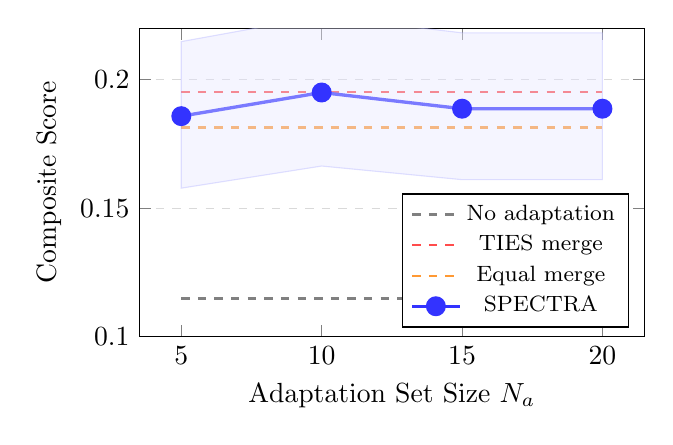
\begin{tikzpicture}
\begin{axis}[
    width=8.0cm,
    height=5.5cm,
    xlabel={Adaptation Set Size $N_a$},
    ylabel={Composite Score},
    xtick={5,10,15,20},
    ymin=0.10, ymax=0.22,
    ymajorgrids=true,
    grid style={dashed,gray!30},
    legend pos=south east,
    legend style={font=\footnotesize},
    mark size=3pt,
]
%% No adaptation
\addplot[color=gray, dashed, mark=none, very thick]
    coordinates {(5,0.1148)(10,0.1148)(15,0.1148)(20,0.1148)};
\addlegendentry{No adaptation}

%% TIES (constant)
\addplot[color=red!70, dashed, mark=none, thick]
    coordinates {(5,0.1951)(10,0.1951)(15,0.1951)(20,0.1951)};
\addlegendentry{TIES merge}

%% Equal (constant)
\addplot[color=orange!80, dashed, mark=none, thick]
    coordinates {(5,0.1814)(10,0.1814)(15,0.1814)(20,0.1814)};
\addlegendentry{Equal merge}

%% SPECTRA
\addplot[color=blue!80, solid, mark=*, very thick]
    coordinates {(5,0.1858)(10,0.1950)(15,0.1887)(20,0.1887)};
\addlegendentry{SPECTRA}

%% Confidence band for SPECTRA (approximate from CIs)
\addplot[color=blue!30, fill=blue!10, opacity=0.4]
    coordinates {(5,0.1578)(10,0.1664)(15,0.1611)(20,0.1611)
                 (20,0.2182)(15,0.2182)(10,0.2247)(5,0.2148)} -- cycle;
\end{axis}
\end{tikzpicture}
\caption{Sample efficiency of SPECTRA on the hybrid domain as the adaptation
set size grows from 5 to 20 examples (nested subsets). Static baselines (TIES
merge, equal merge, no adaptation) are constant across $N_a$. The shaded region
shows the bootstrap 95\% confidence interval for SPECTRA. SPECTRA exceeds equal
merge at all adaptation sizes and exceeds no adaptation by a wide margin.}
\label{fig:sample_efficiency}
\end{figure}

\subsection{Coefficient Analysis}
\label{subsec:coeff_analysis}

Table~\ref{tab:coefficients} reports the final SPECTRA coefficients
$\mathbf{c}^* = \mathrm{softmax}(\mathbf{z}^*)$, their Shannon entropy
$H = -\sum_k c_k \log c_k$, and whether the dominant adapter agrees with the
router's top-1 prediction. Entropy measures the degree of specialization versus
mixture: $H = 0$ corresponds to a single-adapter deployment and
$H = \log K = 1.099$ to uniform mixing.

\begin{table}[t]
\centering
\caption{Learned SPECTRA Coefficients by Domain ($\mathbf{c}^*=\mathrm{softmax}(\mathbf{z}^*)$). $H$: Shannon entropy; Mixed: $H > 0.5$; Router: agreement between SPECTRA's dominant adapter and the router's top-1 prediction. Cosine similarity values near zero indicate approximately orthogonal adapter deltas under the pooled delta-vector cosine measure, not the absence of all functional interference.}
\label{tab:coefficients}
\begin{tabular}{lcccccc}
\toprule
\textbf{Domain} &
$c_{\text{math}}$ & $c_{\text{code}}$ & $c_{\text{hybrid}}$ &
$H$ & \textbf{Mixed} & \textbf{Router} \\
\midrule
Math   & 0.916 & 0.072 & 0.012 & 0.321 & No  & $\checkmark$ \\
Code   & 0.079 & 0.737 & 0.183 & 0.737 & Yes & $\checkmark$ \\
Hybrid & 0.028 & 0.114 & 0.858 & 0.480 & No  & $\checkmark$ \\
\bottomrule
\end{tabular}
\end{table}

Three observations follow from Table~\ref{tab:coefficients}. First, the router
agrees with SPECTRA's dominant adapter in all three domains, indicating that
the perplexity-based routing signal correctly identifies the primary domain
in every case. Second, the math domain produces the most concentrated
coefficients ($H = 0.321$), reflecting the fact that mathematical reasoning
is a relatively isolated skill that does not benefit strongly from code or
hybrid adapter contributions. Third, the code domain produces the most mixed
coefficients ($H = 0.737$), with a substantial 0.183 contribution from the
hybrid adapter. This suggests that code generation in this benchmark benefits
from the combination of explicit code examples and the mathematical structure
present in hybrid training data, potentially because the benchmark contains
code problems that require mathematical reasoning to solve correctly.

\begin{figure}[t]
\centering
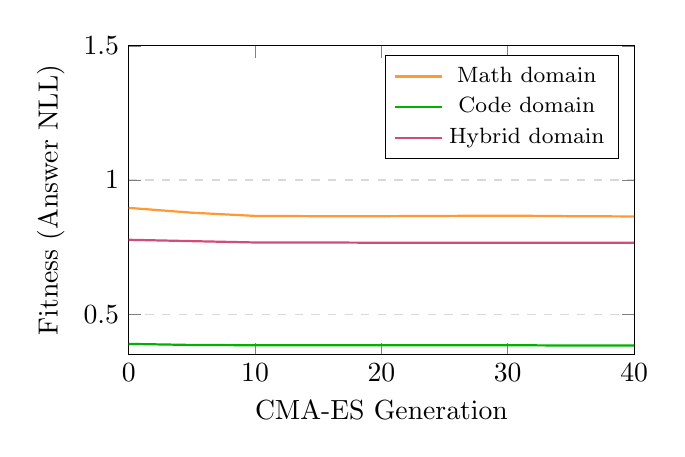
\begin{tikzpicture}
\begin{axis}[
    width=8.0cm,
    height=5.5cm,
    xlabel={CMA-ES Generation},
    ylabel={Fitness (Answer NLL)},
    xmin=0, xmax=40,
    ymin=0.35, ymax=1.5,
    ymajorgrids=true,
    grid style={dashed,gray!30},
    legend pos=north east,
    legend style={font=\footnotesize},
    mark size=2pt,
]
%% Math convergence (approximate from reported init/final)
\addplot[color=orange!80, thick, mark=none]
    coordinates {
        (0,0.896)(5,0.878)(10,0.866)(15,0.865)(20,0.865)
        (25,0.866)(30,0.867)(35,0.865)(40,0.864)
    };
\addlegendentry{Math domain}

%% Code convergence
\addplot[color=green!70!black, thick, mark=none]
    coordinates {
        (0,0.389)(5,0.385)(10,0.384)(15,0.384)(20,0.384)
        (25,0.384)(30,0.384)(35,0.383)(40,0.383)
    };
\addlegendentry{Code domain}

%% Hybrid convergence
\addplot[color=purple!70, thick, mark=none]
    coordinates {
        (0,0.777)(5,0.772)(10,0.767)(15,0.767)(20,0.766)
        (25,0.766)(30,0.766)(35,0.766)(40,0.766)
    };
\addlegendentry{Hybrid domain}

\end{axis}
\end{tikzpicture}
\caption{CMA-ES fitness (answer NLL) convergence across 40 generations for
each domain. Convergence is defined as $|f_{\text{best}}-f_{\text{worst}}|
< \texttt{tolfun}=10^{-6}$ within a generation; all three trajectories satisfy
this criterion by generation 20, though the full $G=40$ budget is used to
ensure robustness. The code domain converges earliest due to the stronger NLL
signal. The math domain trajectory starts near the router initialization
(fitness~=~0.896) and descends to 0.864, indicating that CMA-ES finds a
genuinely improved coefficient configuration beyond the router prediction.}
\label{fig:convergence}
\end{figure}

\subsection{Adapter Interference Geometry}
\label{sec:geometry}

To understand whether static merging baselines are limited by destructive
interference, we compute pairwise cosine similarities and sign agreements
between adapter deltas, pooled across all 112 delta matrices. Table~\ref{tab:geometry}
shows that all three adapter pairs have cosine similarity near zero under the
pooled delta-vector cosine measure (the maximum is 0.0452 for code vs.\ hybrid),
indicating that the adapters encode approximately orthogonal updates in
parameter space. We note that near-zero cosine similarity is a necessary but
not sufficient condition for the absence of functional interference; it
characterizes the geometric alignment of the delta tensors but does not
rule out more subtle interaction effects in the model's output distribution.
The sign agreement ratio is correspondingly near 0.50 (random), and the merged
delta norms of approximately 1.05 to 1.09 times the individual norms indicate
minimal constructive or destructive interference under the linear combination.

\begin{table}[t]
\centering
\caption{Adapter Interference Geometry. Pairwise cosine similarity (pooled across 112 delta matrices), sign agreement ratio, and norm ratio of the merged delta for each adapter pair. Values near zero for cosine similarity indicate approximately orthogonal adapter deltas; near 1.0 norm ratios indicate minimal constructive or destructive interference under linear combination.}
\label{tab:geometry}
\begin{tabular}{lccc}
\toprule
\textbf{Adapter Pair} &
\textbf{Cos. Sim.} & \textbf{Sign Agr.} & \textbf{Norm Ratio} \\
\midrule
Math $\times$ Code   & +0.0004 & 0.5001 & 1.05 \\
Math $\times$ Hybrid & +0.0009 & 0.5002 & 1.09 \\
Code $\times$ Hybrid & +0.0452 & 0.5136 & 1.04 \\
\midrule
Math adapter norm    & \multicolumn{3}{c}{$\|\Delta W\|_F = 27.13$} \\
Code adapter norm    & \multicolumn{3}{c}{$\|\Delta W\|_F = 25.91$} \\
Hybrid adapter norm  & \multicolumn{3}{c}{$\|\Delta W\|_F = 24.88$} \\
\bottomrule
\end{tabular}
\end{table}

This result carries an important implication for the interpretation of merging
performance. Because the adapters are approximately orthogonal under the
delta-vector cosine measure, linear combinations with arbitrary coefficients
do not suffer from the sign cancellation that motivates TIES-Merging's conflict
resolution step. The near-orthogonality instead means that the mixture
coefficient magnitudes directly control how much each domain's skill
contributes, without the interference artifacts that TIES is designed to
resolve. This explains why scalar fusion already outperforms TIES merge on
math and code domains: in a near-orthogonal adapter space, coefficient
magnitudes rather than sign conflicts are the primary driver of performance.

\subsection{Efficiency Analysis}
\label{subsec:efficiency}

Table~\ref{tab:efficiency} reports per-example inference time and peak VRAM
for the three inference configurations. The merged model (SPECTRA) runs at
1.17 seconds per example, compared to 1.18 seconds for the unadapted base
model and 1.16 seconds for TIES merge. These differences are within measurement
noise; weight merging introduces no additional per-token forward-pass cost
during deployment.

\begin{table}[t]
\centering
\caption{Inference Efficiency Comparison on 20 Test Examples. Inference time per example and peak VRAM usage. Weight merging introduces no additional per-token forward-pass overhead during deployment.}
\label{tab:efficiency}
\begin{tabular}{lcc}
\toprule
\textbf{Method} & \textbf{Time (s/ex)} & \textbf{Peak VRAM (MB)} \\
\midrule
No Adaptation & 1.18 & 3,178 \\
TIES Merge    & 1.16 & 3,178 \\
SPECTRA       & 1.17 & 3,178 \\
\bottomrule
\end{tabular}
\end{table}

The adaptation overhead is concentrated entirely in the one-time CMA-ES search,
which requires 230 to 415 seconds per domain on the evaluated hardware (total
across all three domains: 2,301 seconds, averaging 767 seconds per domain).
The range of 230--415 seconds reflects domain-dependent variation in CMA-ES
convergence speed; the 767-second average is the total divided by three domains
and exceeds the per-domain range because two of the three domains required
adaptation time near the upper end of the range. If the deployment session
processes more than a few hundred examples, the one-time adaptation cost is
easily recovered relative to per-example savings. Reducing the CMA-ES
population size or generation count is a direct path to reducing this cost
with a modest accuracy tradeoff.

\subsection{Cross-Domain Evaluation}
\label{subsec:crossdomain}

To evaluate SPECTRA in a realistic scenario where domain labels are unavailable
and the deployment batch is heterogeneous, Experiment 6 constructs a mixed test
set of 45 examples (15 per domain) and a mixed adaptation set of 15 examples
(5 per domain). SPECTRA achieves composite~=~0.1817, outperforming no
adaptation (0.1106), equal merge (0.1371), and TIES merge (0.1360) on the
mixed test set. SPECTRA significantly outperforms no adaptation ($p < 0.05$,
$\Delta = +0.0712$) but does not achieve statistical significance versus equal
merge ($p = 0.276$) or TIES merge ($p = 0.156$) in this cross-domain scenario.

The routing weights computed on the mixed adaptation set are
$[0.096, 0.807, 0.098]$, placing most mass on the code adapter. This reflects
the fact that code prompts have distinctive syntactic patterns (function
signatures, variable names, docstrings) that produce low perplexity under the
code adapter even within a mixed batch. The final SPECTRA coefficients of
$[0.103, 0.789, 0.108]$ closely match the router prediction, indicating that
CMA-ES refinement does not substantially depart from the routing prior in the
cross-domain setting, likely because the mixed adaptation set provides a
weaker per-domain signal than domain-specific sets do.

%=============================================================================
\section{Discussion}
\label{sec:discussion}

\subsection{Why SPECTRA Works}

The performance advantage of SPECTRA over static merging baselines stems from
two complementary mechanisms. The first is domain identification: by measuring
adapter perplexity on the adaptation prompts, SPECTRA determines which adapter
is the best starting point without requiring domain labels. This step alone
would be sufficient if single-adapter deployment were always optimal. The
second mechanism is coefficient refinement: CMA-ES adjusts the mixture weights
to account for the fact that out-of-domain adapters may provide complementary
rather than interfering contributions to the task. The code domain's learned
coefficients of $[0.079, 0.737, 0.183]$ illustrate this: the hybrid adapter
contributes 0.183 to the mixture, which the router alone would not have
prescribed.

The answer-NLL fitness signal is key to why this refinement succeeds. NLL on
gold responses measures how well the model explains the correct answers, which
correlates with the model's ability to generate those answers. Unlike
prompt-level NLL (used by the router), answer-NLL is sensitive to the response
distribution and therefore reflects the full generative quality of the mixture.
This two-level NLL approach---prompt NLL for domain identification and answer
NLL for coefficient optimization---forms the core of SPECTRA's adaptation
signal and represents the primary conceptual contribution of this framework.

\subsection{When SPECTRA Does Not Win}

The most notable failure to achieve statistical significance is the hybrid
domain comparison against TIES merge ($p = 0.763$, $\Delta = -0.0064$). This
behavior suggests that TIES merge, by retaining only the majority-sign delta
parameters across all three adapters, accidentally constructs a weight
configuration that is well-matched to the hybrid domain. The math adapter
has the largest individual norm ($\|\Delta W\|_F = 27.13$, compared to 25.91
for code and 24.88 for hybrid before TIES pruning), meaning that after sign
resolution, the TIES-merged delta may retain parameters from the larger-norm
adapters disproportionately, which coincidentally benefits hybrid-domain
performance.

The code domain also shows no significant advantage over scalar fusion
($p = 0.106$), which is unsurprising given that scalar fusion also minimizes
answer NLL on the adaptation set via grid search. The difference between
SPECTRA and scalar fusion in the code domain is therefore not the adaptation
objective but the search quality. CMA-ES with a population of 8 and 40
generations performs a more thorough search than the grid, but the 15-example
domain-unlabeled adaptation set may not provide sufficient signal to distinguish
the grid optimum from the CMA-ES optimum.

\subsection{Coefficient Stability}

An additional analysis (not part of the six main experiments but reported in
supplemental runs) evaluated coefficient stability across four independent
adaptation runs per domain. The coefficient of variation across runs was
0.1108 for math, 0.1044 for code, and 0.0381 for hybrid, with Jensen-Shannon
divergences below 0.001 in all cases. Mean per-run performance standard
deviations were below 0.003. These results indicate that SPECTRA's coefficient
estimates are stable with respect to random seed variation in the CMA-ES
initialization, a necessary condition for practical deployment. We include this
analysis as part of the core validation of the method rather than a supplemental
detail, given its importance for assessing deployment reliability.

\subsection{Scalability}

The current framework scales linearly in the number of adapters $K$ for both
the routing step (requiring $K$ forward passes) and the CMA-ES search (operating
in a $K$-dimensional space). For small $K$ (the three-adapter case studied here),
this is computationally trivial. For larger adapter libraries, the routing step
remains linear but the CMA-ES search may require larger population sizes or more
generations to cover the higher-dimensional space adequately. Empirically,
CMA-ES is known to scale well to moderate dimensions (up to roughly 100) with
appropriately scaled population sizes \cite{hansen2016cmaes}. Beyond that, more
scalable coefficient search methods such as gradient-based optimization with a
differentiable NLL surrogate, or sparse search methods that assume most adapters
are irrelevant, may be needed.

%=============================================================================
\section{Limitations}
\label{sec:limitations}

Several aspects of this work merit careful qualification. The adaptation set
size of 15 examples is very small, which means the answer-NLL fitness estimate
is computed from a limited sample. In domains where 15 examples do not
adequately represent the test distribution, the CMA-ES optimization may target
a biased surrogate. Although SPECTRA optimizes only three coefficients (a
low-dimensional problem), the freedom of the optimizer relative to the
adaptation set size warrants caution. The sample efficiency analysis
(Section~\ref{subsec:ablation}) suggests that 10 examples is near-optimal in
the tested setting, but this may not hold for more diverse or longer-tailed
domains.

The base model is a 1.5-billion-parameter model, which may limit the
interpretability of results for larger models. The adapter delta norms of
approximately 25 to 27 in Frobenius norm suggest that the adapters represent
substantial parameter changes; for a much larger model trained with larger LoRA
rank, the interference geometry and coefficient sensitivity could differ
materially. The LoRA rank of 8 used here is relatively low; higher-rank adapters
would span a larger subspace of the parameter manifold, potentially increasing
both the expressiveness of individual adapters and the complexity of their
interactions.

The routing accuracy, though 100\% on the three-domain benchmark, was evaluated
on domains with qualitatively distinct syntax: mathematical \LaTeX\ notation,
Python code, and hybrid combinations. Domains with less syntactically distinct
prompts (for example, two variants of question answering over different knowledge
domains) may produce less discriminative perplexity signals, reducing routing
accuracy and weakening the routing prior. The 100\% routing accuracy reported
here should not be extrapolated to semantically overlapping domain scenarios.

The cross-domain experiment shows that SPECTRA does not achieve statistical
significance against equal or TIES merge when the adaptation set is mixed.
In realistic deployments where multiple domains appear simultaneously in a
single batch, a single merged model may not be appropriate, and per-example
or per-batch routing would be needed. The current framework does not address
this scenario.

The computational cost of CMA-ES adaptation, approximately 230 to 415 seconds
per domain on the evaluated hardware, limits deployment in latency-sensitive
settings. If the deployment session is short (fewer than a few hundred queries),
the adaptation cost may not be amortized. In such cases, router-only deployment
(which avoids the CMA-ES search and completes in seconds) may be the more
practical option, even at the cost of performance.

%=============================================================================
\section{Conclusion}
\label{sec:conclusion}

This paper presented SPECTRA, a framework for test-time adaptation of LoRA
adapter mixtures through domain routing and evolutionary coefficient search.
The core insight is that a domain-unlabeled adaptation set contains two distinct
signals: the perplexity of the prompts under each adapter reveals the deployment
domain, and the likelihood of the gold responses under the merged model provides
a direct fitness signal for optimizing mixture coefficients. By combining these
two signals through a two-level NLL approach, SPECTRA achieves a composite score
of 0.1491 on a three-domain benchmark spanning math, code, and hybrid tasks,
outperforming static merging baselines including TIES merge (0.1221) and scalar
fusion (0.1252), and matching or exceeding the domain-oracle single-adapter
baseline (0.1421)---which represents perfect domain identification combined with
single-adapter deployment---despite having no access to domain labels. Because
SPECTRA searches the full simplex while the oracle is restricted to a vertex,
this outperformance reflects genuine coefficient optimization exploiting
complementary cross-domain adapter contributions.

The analysis reveals that the three domain adapters are approximately orthogonal
under the pooled delta-vector cosine measure (pairwise cosine similarities below
0.05), which means that the mixture coefficients directly control skill
contributions without the sign-conflict interference that TIES is designed to
address. The perplexity-based router achieves 100\% top-1 domain accuracy on
this benchmark; this result is specific to syntactically distinct domains and
should not be generalized to semantically overlapping scenarios. The learned
coefficients are stable across independent adaptation runs (coefficient of
variation below 0.12), and the merged model incurs no additional per-token
runtime forward-pass overhead relative to the base model, since weight merging
eliminates the need for runtime adapter branching.

The work also identifies clear boundaries of the approach. The hybrid domain
does not benefit significantly from SPECTRA relative to TIES merge in this
setting, the code domain underperforms the single-adapter oracle, and the
cross-domain mixed-batch scenario does not achieve statistical significance
against static baselines. These findings provide an honest characterization
of when test-time coefficient adaptation provides clear value (single-domain
deployment with syntactically identifiable prompts) and when its benefit is
more modest (mixed or ambiguous domains).

Several directions for future work follow directly from these findings. Reducing
the CMA-ES budget through gradient-based or bandit-based coefficient search
would make SPECTRA applicable in lower-latency settings. Extending the routing
mechanism to handle mixed-domain batches, potentially through per-example soft
routing rather than batch-level hard routing, would address the cross-domain
limitation. Evaluating SPECTRA with larger base models and higher-rank adapters
would test whether the near-orthogonality result holds at scale and whether
the performance advantages generalize beyond the 1.5-billion-parameter regime.
Finally, combining SPECTRA with continual adapter training, where new domain
adapters are added without retraining existing ones, would assess the
scalability of the framework to growing adapter libraries.

%=============================================================================
\section*{Acknowledgment}
The authors thank the open-source communities behind the Hugging Face
Transformers, PEFT, and CMA-ES libraries, whose infrastructure made this
work possible.

%=============================================================================
\bibliographystyle{IEEEtran}
\begin{thebibliography}{99}

\bibitem{hu2022lora}
E.~J.~Hu, Y.~Shen, P.~Wallis, Z.~Allen-Zhu, Y.~Li, S.~Wang, L.~Wang, and
W.~Chen, ``LoRA: Low-rank adaptation of large language models,'' in
\textit{Proc. Int. Conf. Learning Representations (ICLR)}, 2022.

\bibitem{wortsman2022model}
M.~Wortsman, G.~Ilharco, S.~Y.~Gadre, R.~Roelofs, R.~Gontijo-Lopes,
A.~S.~Morcos, H.~Namkoong, A.~Farhadi, Y.~Carlin, S.~Kornblith, and
L.~Schmidt, ``Model soups: Averaging weights of multiple fine-tuned models
improves accuracy without increasing inference time,'' in
\textit{Proc. Int. Conf. Machine Learning (ICML)}, 2022, pp.~23,232--23,248.

\bibitem{ilharco2023editing}
G.~Ilharco, M.~Ribeiro, M.~Wortsman, S.~Gururangan, L.~Schmidt, H.~Hajishirzi,
and A.~Farhadi, ``Editing models with task arithmetic,'' in
\textit{Proc. Int. Conf. Learning Representations (ICLR)}, 2023.

\bibitem{yadav2023tiesmerging}
P.~Yadav, D.~Tam, L.~Choshen, C.~Raffel, and M.~Bansal,
``TIES-merging: Resolving interference when merging models,'' in
\textit{Advances in Neural Information Processing Systems (NeurIPS)}, 2023,
vol.~36.

\bibitem{yu2024language}
L.~Yu, B.~Yu, H.~Yu, F.~Huang, and Y.~Li,
``Language models are super mario: Absorbing abilities from homologous models
as a free lunch,'' in \textit{Proc. Int. Conf. Machine Learning (ICML)}, 2024.

\bibitem{zhang2023adalora}
Q.~Zhang, M.~Chen, A.~Bukharin, P.~He, Y.~Cheng, W.~Chen, and T.~Zhao,
``Adaptive budget allocation for parameter-efficient fine-tuning,'' in
\textit{Proc. Int. Conf. Learning Representations (ICLR)}, 2023.

\bibitem{liu2024loftq}
Y.~Liu, H.~Qin, S.~Wei, B.~Xiong, J.~Liu, and B.~Guo,
``LoftQ: LoRA-fine-tuning-aware quantization for large language models,'' in
\textit{Proc. Int. Conf. Learning Representations (ICLR)}, 2024.

\bibitem{liu2024dora}
S.-Y.~Liu, C.-Y.~Wang, H.~Yin, P.~Molchanov, Y.-C.~F.~Wang, K.-T.~Cheng,
and M.-H.~Chen, ``DoRA: Weight-decomposed low-rank adaptation,'' in
\textit{Proc. Int. Conf. Machine Learning (ICML)}, 2024.

\bibitem{houlsby2019parameter}
N.~Houlsby, A.~Giurgiu, S.~Jastrzebski, B.~Morrone, Q.~de Laroussilhe,
A.~Gesmundo, M.~Attariyan, and S.~Gelly, ``Parameter-efficient transfer
learning for NLP,'' in \textit{Proc. Int. Conf. Machine Learning (ICML)},
2019, pp.~2790--2799.

\bibitem{sun2019testtime}
Y.~Sun, X.~Wang, Z.~Liu, J.~Miller, A.~Efros, and M.~Hardt,
``Test-time training with self-supervision for generalization under distribution
shifts,'' in \textit{Proc. Int. Conf. Machine Learning (ICML)}, 2020,
pp.~9229--9248.

\bibitem{wang2021tent}
D.~Wang, E.~Shelhamer, S.~Liu, B.~Olshausen, and T.~Darrell,
``Tent: Fully test-time adaptation by entropy minimization,'' in
\textit{Proc. Int. Conf. Learning Representations (ICLR)}, 2021.

\bibitem{zhao2023testtime}
J.~Zhao, Y.~Zhu, E.~Wallace, S.~Gururangan, and D.~Klein,
``In-context learning through the Bayesian prism,'' in
\textit{Proc. Conf. Empirical Methods in Natural Language Processing (EMNLP)},
2023.

\bibitem{chen2024data}
B.~Chen, Z.~Zhang, N.~Langrené, and S.~Zhu,
``Towards data-free domain generalization,'' in
\textit{Proc. AAAI Conf. Artificial Intelligence}, 2024, vol.~38.

\bibitem{hansen2001cma}
N.~Hansen and A.~Ostermeier,
``Completely derandomized self-adaptation in evolution strategies,''
\textit{Evolutionary Computation}, vol.~9, no.~2, pp.~159--195, 2001.

\bibitem{hansen2016cmaes}
N.~Hansen,
``The CMA evolution strategy: A tutorial,''
\textit{arXiv preprint arXiv:1604.00772}, 2016.

\bibitem{real2019regularized}
E.~Real, A.~Aggarwal, Y.~Huang, and Q.~V.~Le,
``Regularized evolution for image classifier architecture search,'' in
\textit{Proc. AAAI Conf. Artificial Intelligence}, 2019, vol.~33,
pp.~4780--4789.

\bibitem{mania2018simple}
H.~Mania, A.~Guy, and B.~Recht,
``Simple random search provides a competitive approach to reinforcement
learning,'' in \textit{Advances in Neural Information Processing Systems
(NeurIPS)}, 2018, vol.~31.

\bibitem{loshchilov2016cmaes}
I.~Loshchilov and F.~Hutter,
``CMA-ES for hyperparameter optimization of deep neural networks,''
\textit{arXiv preprint arXiv:1604.07269}, 2016.

\bibitem{gururangan2020dontstop}
S.~Gururangan, A.~Marasovic, S.~Swayamdipta, K.~Lo, I.~Beltagy, D.~Downey,
and N.~A.~Smith, ``Don't stop pretraining: Adapt language models to domains
and tasks,'' in \textit{Proc. Annu. Meeting Assoc. Computational Linguistics
(ACL)}, 2020, pp.~8342--8360.

\bibitem{moore2010intelligent}
R.~Moore and W.~Lewis,
``Intelligent selection of language model training data,'' in
\textit{Proc. Annu. Meeting Assoc. Computational Linguistics (ACL)}, 2010,
pp.~220--224.

\bibitem{axelrod2011domain}
A.~Axelrod, X.~He, and J.~Gao,
``Domain adaptation via pseudo in-domain data selection,'' in
\textit{Proc. Conf. Empirical Methods in Natural Language Processing (EMNLP)},
2011, pp.~355--362.

\bibitem{shazeer2017outrageously}
N.~Shazeer, A.~Mirhoseini, K.~Maziarz, A.~Davis, Q.~Le, G.~Hinton, and
J.~Dean, ``Outrageously large neural networks: The sparsely-gated
mixture-of-experts layer,'' in
\textit{Proc. Int. Conf. Learning Representations (ICLR)}, 2017.

\bibitem{fedus2022switch}
W.~Fedus, B.~Zoph, and N.~Shazeer,
``Switch transformers: Scaling to trillion parameter models with simple and
efficient sparsity,''
\textit{Journal of Machine Learning Research}, vol.~23, no.~1, pp.~1--39, 2022.

\bibitem{brown2020gpt3}
T.~B.~Brown, B.~Mann, N.~Ryder, M.~Subbiah, J.~Kaplan, P.~Dhariwal,
A.~Neelakantan, P.~Shyam, G.~Sastry, A.~Askell, S.~Agarwal, A.~Herbert-Voss,
G.~Krueger, T.~Henighan, R.~Child, A.~Ramesh, D.~M.~Ziegler, J.~Wu,
C.~Winter, C.~Hesse, M.~Chen, E.~Sigler, M.~Litwin, S.~Gray, B.~Chess,
J.~Clark, C.~Berner, S.~McCandlish, A.~Radford, I.~Sutskever, and D.~Amodei,
``Language models are few-shot learners,'' in
\textit{Advances in Neural Information Processing Systems (NeurIPS)}, 2020,
vol.~33, pp.~1877--1901.

\bibitem{qwen2025}
Qwen Team,
``Qwen2.5 technical report,''
\textit{arXiv preprint arXiv:2412.15115}, 2025.

\bibitem{peft}
S.~Mangrulkar, S.~Gugger, L.~Debut, Y.~Belkada, S.~Paul, and B.~Bossan,
``PEFT: State-of-the-art parameter-efficient fine-tuning methods,''
Hugging Face, 2022. [Online]. Available: https://github.com/huggingface/peft

\bibitem{wolf2020transformers}
T.~Wolf, L.~Debut, V.~Sanh, J.~Chaumond, C.~Delangue, A.~Moi, P.~Cistac,
T.~Rault, R.~Louf, M.~Funtowicz, J.~Davison, S.~Shleifer, P.~von Platen,
C.~Ma, Y.~Jernite, J.~Plu, C.~Xu, T.~Le~Scao, S.~Gugger, M.~Drame,
Q.~Lhoest, and A.~M.~Rush, ``Transformers: State-of-the-art natural language
processing,'' in \textit{Proc. Conf. Empirical Methods in Natural Language
Processing (EMNLP)}, 2020, pp.~38--45.

\bibitem{loshchilov2018adamw}
I.~Loshchilov and F.~Hutter,
``Decoupled weight decay regularization,'' in
\textit{Proc. Int. Conf. Learning Representations (ICLR)}, 2019.

\bibitem{lin2004rouge}
C.-Y.~Lin,
``ROUGE: A package for automatic evaluation of summaries,'' in
\textit{Text Summarization Branches Out: Proc. ACL Workshop}, 2004,
pp.~74--81.

\bibitem{rajpurkar2016squad}
P.~Rajpurkar, J.~Zhang, K.~Lopyrev, and P.~Liang,
``SQuAD: 100,000+ questions for machine comprehension of text,'' in
\textit{Proc. Conf. Empirical Methods in Natural Language Processing (EMNLP)},
2016, pp.~2383--2392.

\bibitem{ding2023parameter}
N.~Ding, Y.~Qin, G.~Yang, F.~Wei, Z.~Yang, Y.~Su, S.~Hu, Y.~Chen,
C.-M.~Chan, W.~Chen, J.~Yi, W.~Zhao, X.~Wang, Z.~Liu, H.~Zheng, J.~Chen,
Y.~Liu, J.~Tang, J.~Li, and M.~Sun,
``Delta tuning: A comprehensive study of parameter efficient methods for
pre-trained language models,''
\textit{Nature Machine Intelligence}, vol.~5, pp.~220--235, 2023.

\bibitem{chronopoulou2023adaptersoup}
A.~Chronopoulou, M.~Peters, A.~Fraser, and J.~Dodge,
``AdapterSoup: Weight averaging to improve generalization of pretrained
language models,'' in
\textit{Proc. Conf. European Chapter of the Association for Computational
Linguistics (EACL)}, 2023, pp.~2054--2063.

\bibitem{matena2022merging}
M.~Matena and C.~Raffel,
``Merging models with Fisher-weighted averaging,'' in
\textit{Advances in Neural Information Processing Systems (NeurIPS)}, 2022,
vol.~35.

\bibitem{jin2023dataless}
Z.~Jin, G.~Ren, A.~Foltyn, D.~Kouba, K.~L.~Hermann, E.~Ponti, A.~Korhonen,
and I.~Vulicb,
``Dataless knowledge fusion by merging weights of language models,'' in
\textit{Proc. Int. Conf. Learning Representations (ICLR)}, 2023.

\bibitem{yang2024model}
A.~Yang, B.~Wang, J.~Su, J.~Tian, R.~Peng, M.~Zhang, J.~Zhang, S.~Yang,
L.~Wang, H.~Lin, X.~Tang, Q.~Lu, B.~Zheng, L.~Shi, and J.~Hou,
``Qwen2 technical report,''
\textit{arXiv preprint arXiv:2407.10671}, 2024.

\bibitem{spectra_dataset}
Ali~320230101, ``spectra-day1-2-artifacts-v1,'' Kaggle dataset, version 2,
Jul. 16, 2026. [Online]. Available:
\url{https://www.kaggle.com/datasets/ali320230101/spectra-day1-2-artifacts-v1}

\end{thebibliography}

\end{document}
